\documentclass[11pt,letterpaper,titlepage,en-US]{article}

\usepackage{basicstyle}
\usepackage{homework}
%
% Homework Details
%   - Title
%   - Due date
%   - Class
%   - Section/Time
%   - Instructor
%   - Author
%

\newcommand{\hmwkTitle}{Homework\ \#4 }
\DTMsavetimestamp{DueDate}{2016-11-28T23:59:59-06:00}
\newcommand{\hmwkClass}{CS 6363.005}
\newcommand{\hmwkClassName}{Design and Analysis of Computer Algorithms}
\newcommand{\hmwkClassInstructor}{Instructor: Benjamin Raichel}
\newcommand{\hmwkAuthorName}{Hanlin He}
\newcommand{\hmwkAuthorNetID}{hxh160630}
\newcommand{\hmwkAuthorUTDEmail}{\href{mailto:hanlin.he@utdallas.edu}{hanlin.he@utdallas.edu}}


%
% Title Page
%

\title{
    \vspace{2in}
    \textmd{\textbf{\hmwkClassName \\\hmwkClass:\ \hmwkTitle}}\\
    \normalsize\vspace{0.1in}\small{Due\ on\ \DTMusedate{DueDate}\ at \DTMusetime{DueDate} }\\
    \vspace{0.1in}\large{\textit{\hmwkClassInstructor}}
    \vspace{3in}
}

\author{\textbf{\hmwkAuthorName\ \footnotesize{(\hmwkAuthorNetID)}} \\  \hmwkAuthorUTDEmail}
\date{}
\makeindex

\begin{document}
\maketitle

\pagenumbering{Roman}

\tableofcontents

\pagebreak
\pagenumbering{arabic}


\begin{homeworkProblem}
\begin{homeworkSubProblem}

\begin{figure}[ht!]
    \caption{Example}\label{p4a}
    \centering
    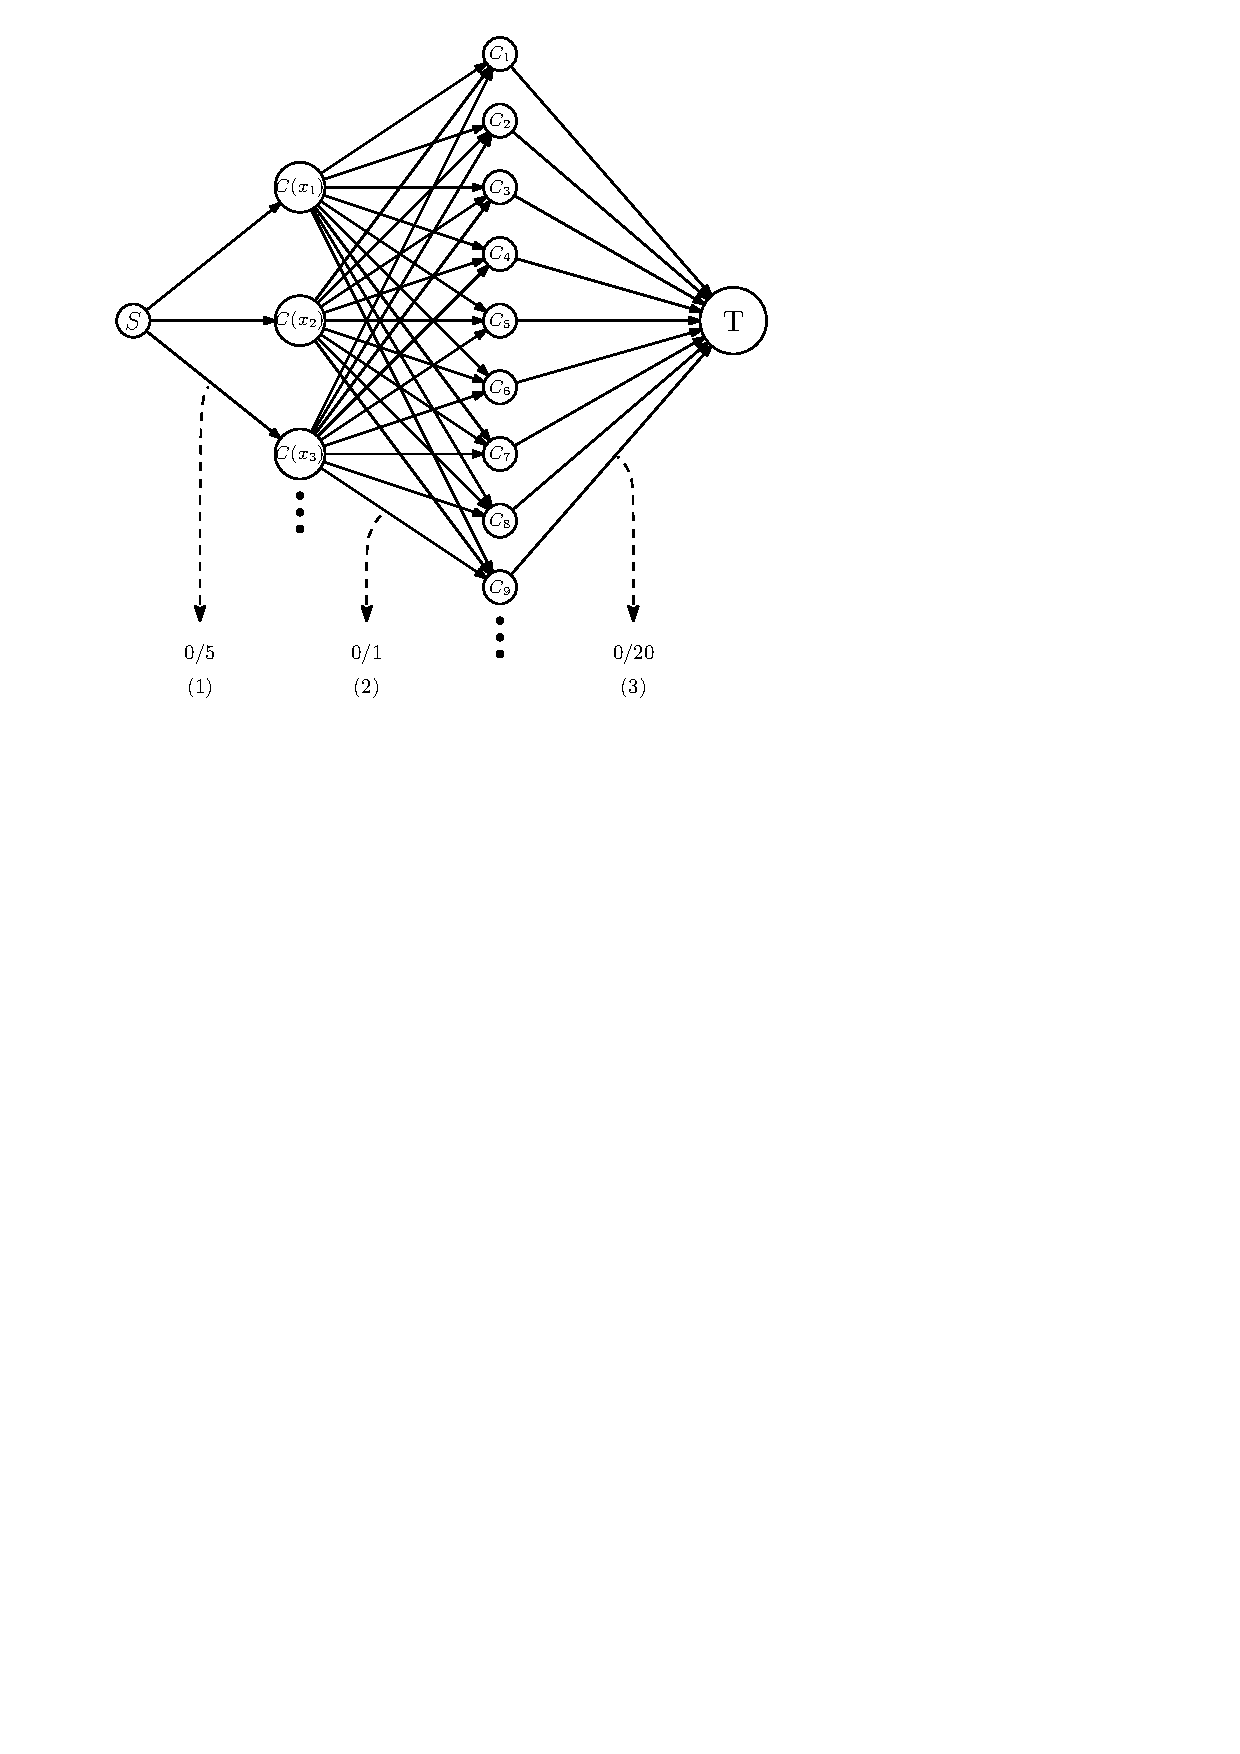
\includegraphics[width=.8\textwidth]{p4a}
\end{figure}
\end{homeworkSubProblem}
\end{homeworkProblem}

\begin{homeworkProblem}
\begin{homeworkSubProblem}
    \bigO{nb} time does not imply $P=NP$, since $b$ is not polynomial in the length of the input
    to the problem.\footnote{Cited from Wikipedia:
    \href{https://en.wikipedia.org/wiki/Knapsack_problem}{Knapsack Problem}}
\end{homeworkSubProblem}

\begin{homeworkSubProblem}
Use the idea of binary search.

Let \ProcedureName{Independent-Set}{G,k} return \textsc{True} if exist
an independent set of size greater than $k$, otherwise return \textsc{False}.

Search the max value in $[0 \ldots k]$.
First try $k/2$, if \ProcedureName{Independent-Set}{G,k/2} = \textsc{True},
call \ProcedureName{Independent-Set}{G, (k + k/2)/2},
otherwise 
call \ProcedureName{Independent-Set}{G, (0 + k/2)/2},
and recursively continue.
Stop until \textsc{True} is returned,
or has made $\lceil\log k\rceil$ recursive calls.

\end{homeworkSubProblem}

\begin{homeworkSubProblem}
Reduce 3SAT to 4SAT:

Change every 3CNF formula into a 4CNF formula.
\[a \lor b \lor c \longrightarrow (a \lor b \lor c \lor x) \land (a \lor b \lor c \lor \overline{x})\]

For each 3CNF formula of $n$ size, there is at most $\binom{n}{3}$ types of clauses.
So this operation takes \bigO{n^3} time ( polynomial time ).

Thus, a 3SAT is reduced to a 4SAT problem, plus a polynomial time operation.

By definition, 3SAT is a NP-hard problem. Hence, we conclude 4SAT is NP-hard.
And because 4SAT is a special case of 3SAT, it is also in NP.
Therefore, 4SAT is NP-complete.
\end{homeworkSubProblem}

\begin{homeworkSubProblem}

\end{homeworkSubProblem}

\end{homeworkProblem}
\end{document}
